\documentclass{article}[a4paper]
\usepackage
[
        a4paper,% other options: a3paper, a5paper, etc
        left=1.5cm,
        right=1.5cm,
        top=2cm,
        bottom=2cm,
        % use vmargin=2cm to make vertical margins equal to 2cm.
        % us  hmargin=3cm to make horizontal margins equal to 3cm.
        % use margin=3cm to make all margins  equal to 3cm.
]
{geometry}

\usepackage[english]{babel}
\usepackage{booktabs, graphicx}   %replacing \hline
\usepackage{longtable}  % formatting tables
\usepackage{dcolumn}    %centering based on dots
\usepackage[utf8]{inputenc}
\usepackage{adjustbox}
\usepackage{blkarray}

\usepackage[colorlinks,linkcolor=blue]{hyperref} % For cross-reference
\usepackage{amsmath,amsfonts,amssymb,amsthm} % For mathematics
\usepackage{float}    % For include graphics
\usepackage{caption,subfigure}

%belows are for highlighting codes
\usepackage{listings}
\usepackage{xcolor}
\usepackage{textcomp}
\usepackage[framed,numbered,autolinebreaks,useliterate]{mcode}
\usepackage[section]{placeins}
\setlength{\parindent}{4 pt}

%if seperate: select specific section.tex:
% \includeonly{file1,file2}

\title{Quant Macro PS5 - Solving the ABHI Model}
\author{Weimin Zhou}
\begin{document}
\maketitle
\begin{abstract}
	Quantitative Macroeconomics Problem Set 5 as a final project.
	the question in \textbf{II Solving the ABHI model} is based on \textbf{I A simple wealth model} which is described on PS5.pdf. 
\end{abstract}

\tableofcontents

\pagebreak 

\section{II.1. The recursive formulation.}
\textbf{\textit{Formulate the problem of the agent recursively, i.e. write down Bellman equation and derive the
stochastic Euler equation.}}.

Bellman Equation is simply just:
\begin{equation}
V(a, y)  = \max_{c} u(c) + \beta E \{ V'(a',y')\}
\end{equation}

And for computational expression, I use: ($w_t$ = 1 by normalization)
\begin{align}
V_t (a_t, y_t)  = \max_{c_t} u(c_t) + \beta E_t \{ V_{t+1}(a_{t+1},y_{t+1})\} \\
\text{s.t. } c_t + a_{t+1} = w_t y_t + (1+r_t) a_t
\end{align}

Solving above maximization problem yield the stochastic Euler equation:

\begin{equation}
u'(c_t)  = E_t \beta (1+r_{t+1})u'(c_{t+1}) = \sum_{y_{t+1}|y_t} \beta (1+r_{t+1}) u'(c_{t+1}(y_{t+1}))
\end{equation}

\section{II.2; II.3; II.4 Algorithm and STEPs}

This part of solution contains in the following matlab .m file respectively:

% Please add the following required packages to your document preamble:
% \usepackage{booktabs}
\begin{table}[]
\centering
\begin{tabular}{@{}lll@{}}
\toprule
  & Matlab File Name                 & Instructions                                        \\ \midrule
1 & infinitely.m                     & Infinite-lived Household problems                   \\
2 & finite\_CRRA\_uncertainty.m      & Finite case, CRRA utility, with uncertainty         \\
3 & finite\_CRRA\_certainty.m        & Finite case, CRRA utility, without uncertainty      \\
4 & finite\_Quadratic\_uncertainty.m & Finite case, Quadratic utility, with uncertainty    \\
5 & finite\_Quadratic\_certainty.m   & Finite case, Quadratic utility, without uncertainty \\ 
6 & II4\_2\_3\_sigma2\_5\_20.m            & Specially for II.4.2 - Q3 compare different $\sigma$\\ \bottomrule
\end{tabular}
\end{table}

For different set up of parameters, I go through the following steps.

\subsection{STEP.1 Generating state space}

For discrete methods, I generate the evenly spaced grids and do VFI. when agents encounter Natural borrowing limit, the utility will reach a large negative value, and in this case, I didn't see. Thus I comment and ignore the case for imposing natural borrowing limit as $a_0$ and $a_T$ for infinite and finite case respectively.

For continuous methods, I use piecewise cubic spline for the nodes and VFI
\subsubsection{Discrete Method}
\[ A \times Y = \{ (a,y): a\in A \text{ and } y\in Y  \}\]

where, $A={a_1, \dots, a_n}$ and $Y = {y_1, y_2}$ with $a_1 = -A$ and use value function or Euler equation methods. Make sure that you define the grid wide enough, i.e. for the last point in the grid $a_n$ it should be the case that $a'(a_n, y_2)<a_n$

\subsubsection{Continuous Method}
suggest to start with piecewise linear splines (there will be potential kinks in the decision rules). Also include in your program a subroutine that simulates paths of consumption and asset holdings for the first 45 periods of an agents life, starting from arbitrary asset position $a_o \in A$ and $y_o \in Y$

\subsection{STEP.2 VFI and simulation paths of consumption and asset holding}

\subsubsection{Infinitely-lived household economy}
I generate a larger enough period (T=10000) to expect the convergence of Value function. 
\subsubsection{The life-cycle economy}
make a finite period (T=45) and do iterate backwards from $v_{t+1}(a,y)=0$.

\section{II.4 solution}

\subsection{II.4.1 No uncertainty: $\gamma=0, \sigma_y = 0 $}
\subsection{1. infinite case}
\textbf{For T = 1 plot the consumption function(s). On the x-axis should be $a$, on the y-axis $c(a, y_1)$ and $c(a,y_2)$ for both preference specifications. Also generate a time profile of consumption by choosing $a_0$ as starting assets and by using the policy functions $c(a,y)$ and $a'(a,y)$.}



\begin{figure}[htbp]
\centering
\begin{minipage}[t]{0.48\textwidth}
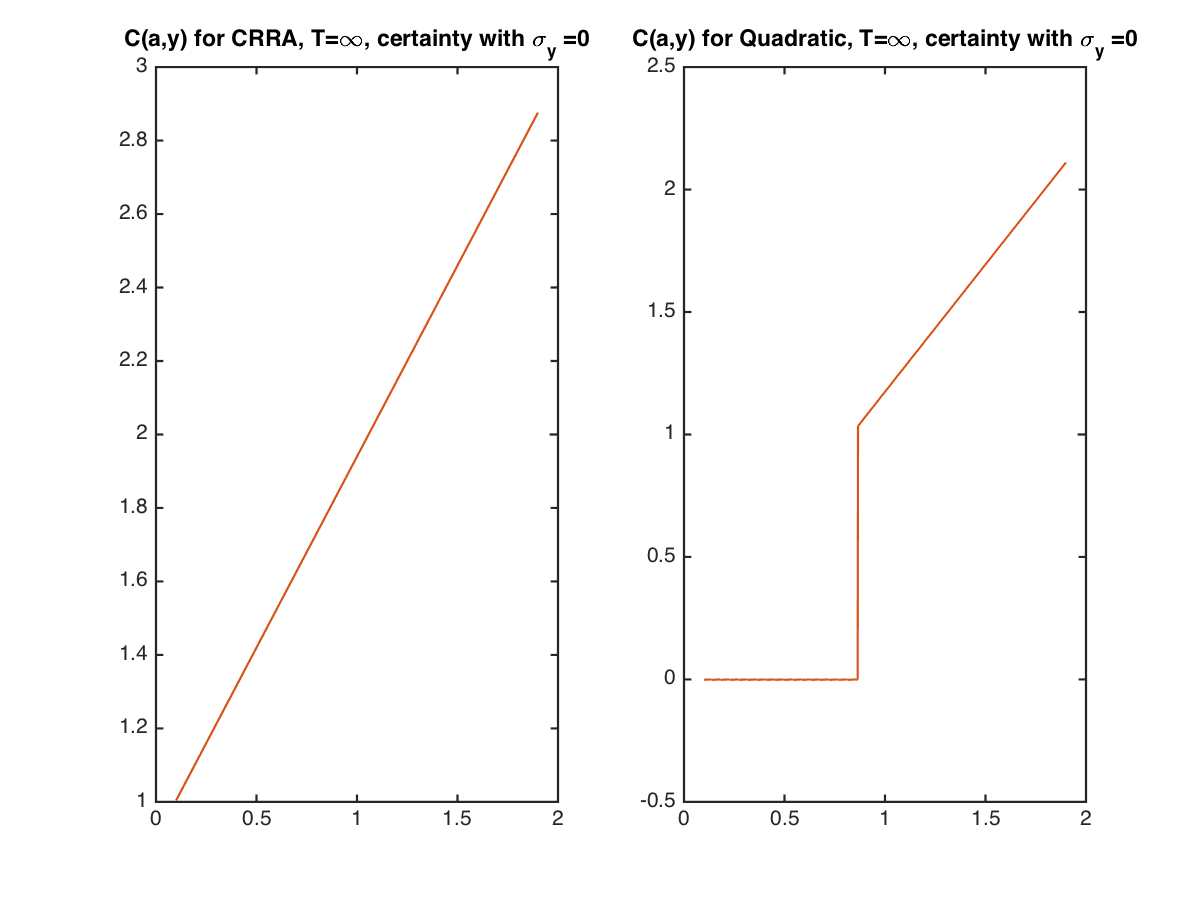
\includegraphics[width=\textwidth]{img/41a.png}
\caption{$T=\infty, c(a,y)$ for two utility functions}\label{Fig1}
\end{minipage}
\begin{minipage}[t]{0.48\textwidth}
\centering
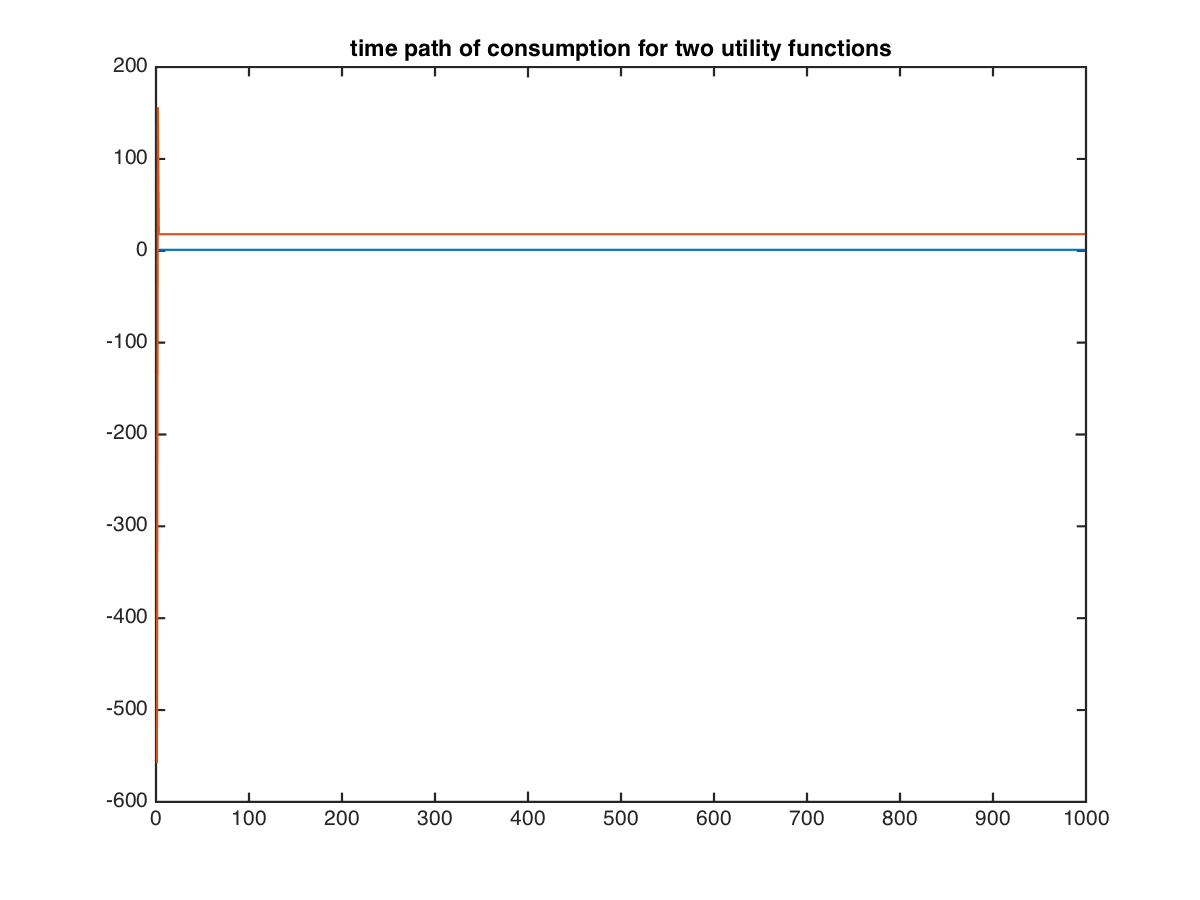
\includegraphics[width=\textwidth]{img/41aa.png}
\caption{Q4-1b}\label{Fig2}
\end{minipage}
\end{figure}


Since Natural borrowing constraint is not binding (running codes display a TRUE return.) hence, under certainty, we should have consumption smooth over all period as discussed in class, which refers to Figure \ref{Fig1}. (with income increase, savings also increase, that's so called precautionary savings due to incompleteness). 

Besides, by requirement, I also attached Figure \ref{Fig2}, denoting the smooth consumption decision. 

\medskip


\subsection{2. finite case}

\textbf{Do the same as in the previous question, but now with T = 45. For the consumption function plots pick two ages, say plot $c_5(a, y)$ and $c_{40}(a, y)$.}

\subsubsection*{CRRA utility}

\begin{figure}[htbp]
\centering
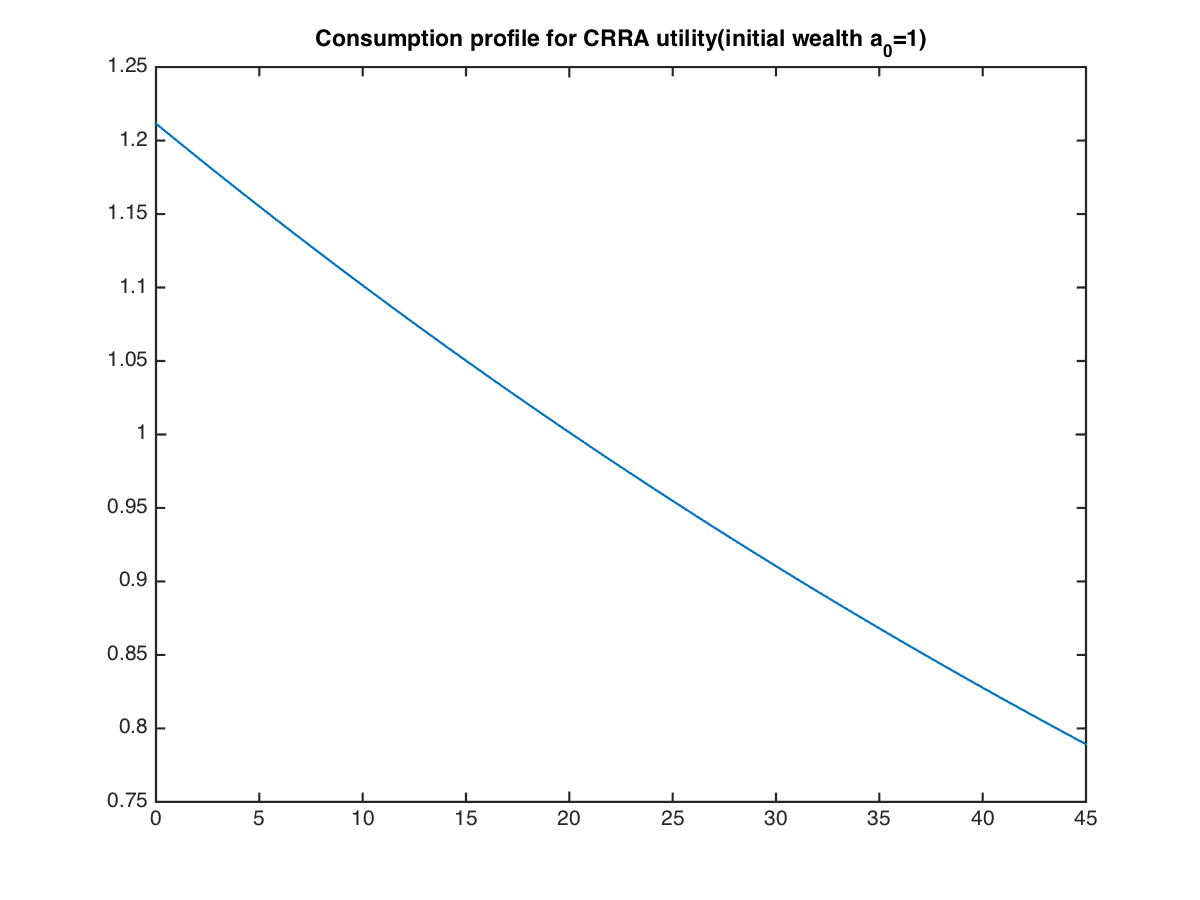
\includegraphics[width=0.68\textwidth]{img/41b.png}
\caption{Q4-1a} \label{fig41b}
\end{figure}


\begin{figure}[htbp]
\centering
\begin{minipage}[t]{0.48\textwidth}
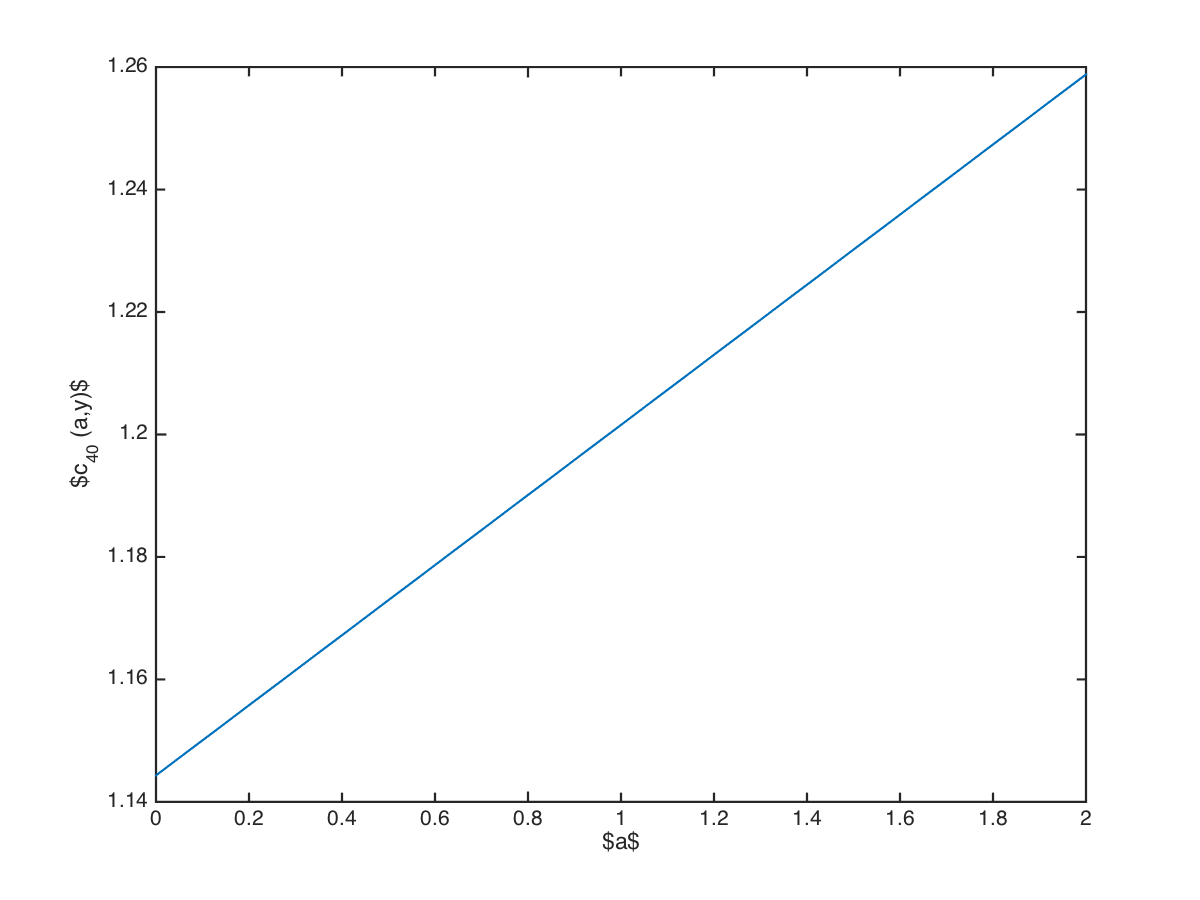
\includegraphics[width=\textwidth]{img/41c.png}
\caption{Q4-1c} \label{fig41c}
\end{minipage}
\begin{minipage}[t]{0.48\textwidth}
\centering
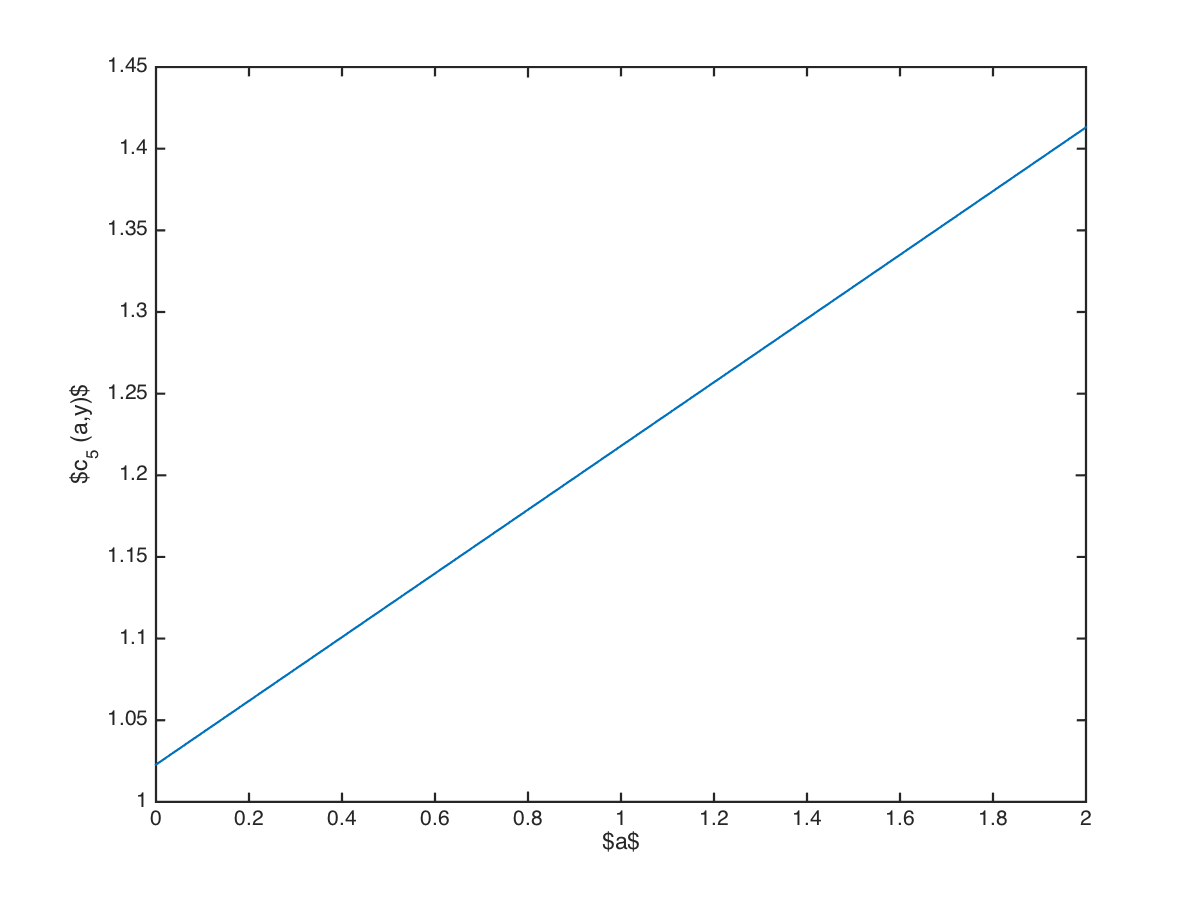
\includegraphics[width=\textwidth]{img/41d.png}
\caption{Q4-1d} \label{fig41d}
\end{minipage}
\end{figure}


In the finite case, I consider again, two utility functions, CRRA and Quadratic forms, in the finite case, as discussed in the class, agents in different age would encounter different decision (hence, we need to plot the Figure \ref{fig41c} and Figure \ref{fig41c}. ) 

Also, I plot the time path of consumption profile, referring to Figure \ref{fig41b}. 

Note: due to the time limit, graph is not so beautiful.

\subsubsection*{Quadratic utility}

\begin{figure}[htbp]
\centering
\begin{minipage}[t]{0.48\textwidth}
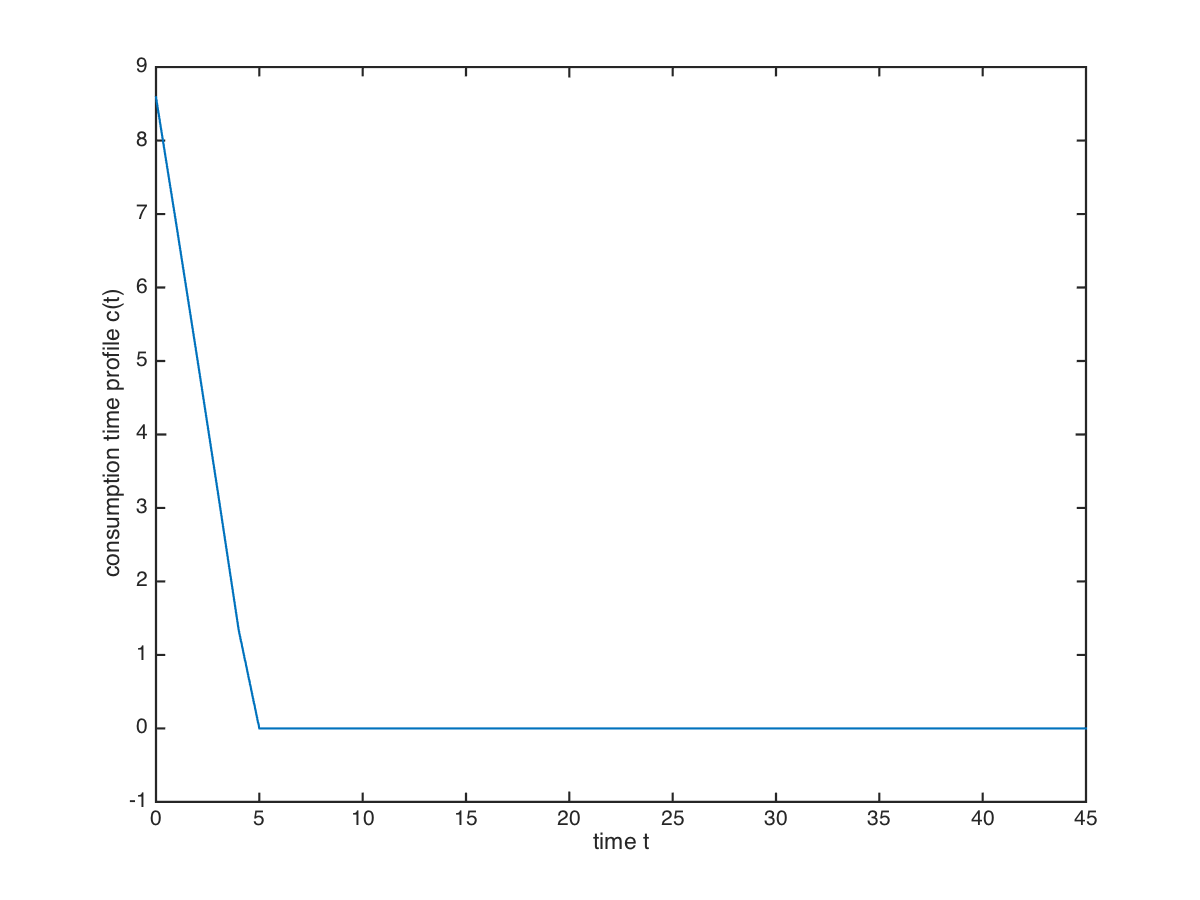
\includegraphics[width=\textwidth]{img/42a.png}
\caption{Consumption time profile for Quadratic Utility}\label{fig42a}
\end{minipage}
\begin{minipage}[t]{0.48\textwidth}
\centering
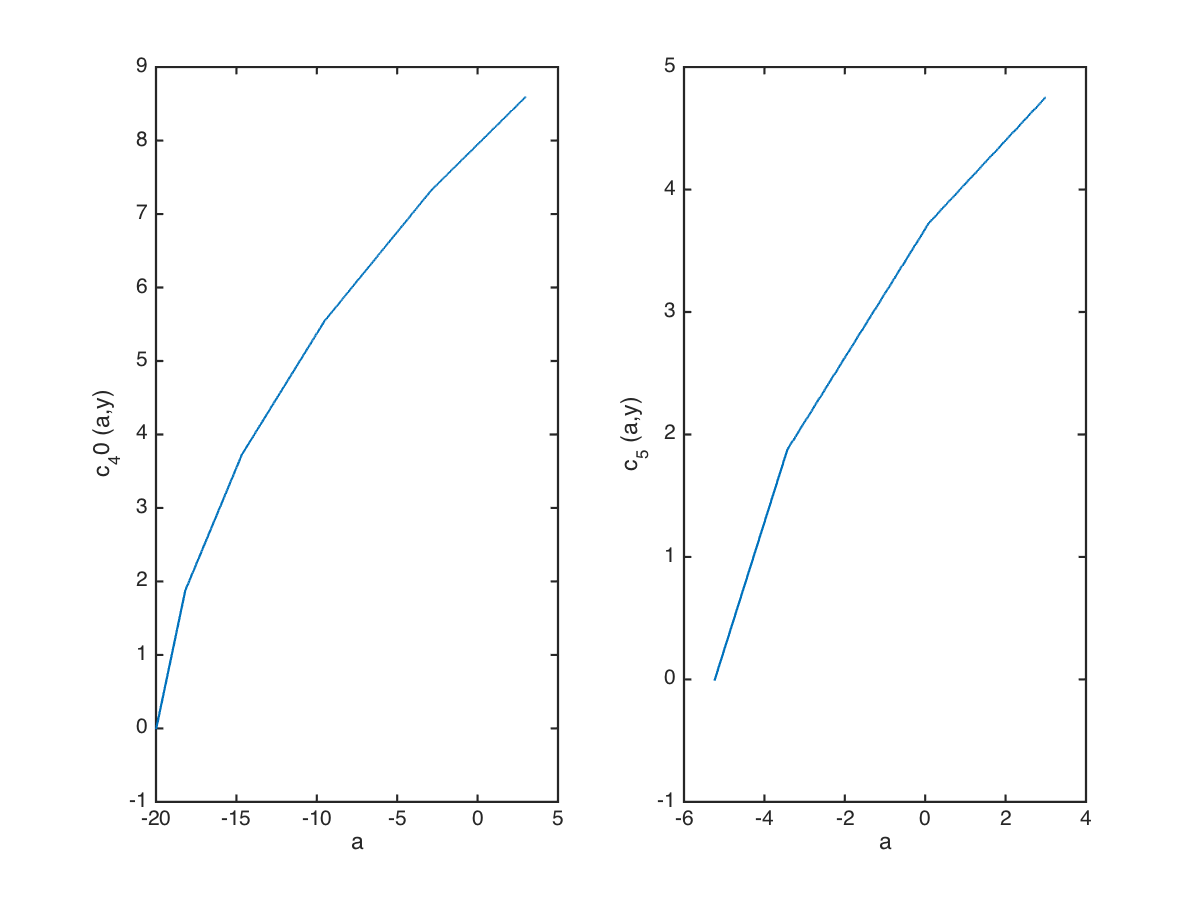
\includegraphics[width=\textwidth]{img/42b.png}
\caption{different-age consumption decision for Quadratic Utility(T=40, T=5)}\label{fig42b}
\end{minipage}
\end{figure}

Similarly with above, by deriving Quadratic function and solve the foc problem, we could obtain below figures (Figure \ref{fig42a} and Figure \ref{fig42b}). 
\pagebreak

\subsection{II.4.2 Uncertainty: $\gamma=0, \sigma_y = 0.1 $}

\subsubsection{1. plot infinitely and finite case of consumption policy function w.r.t state under two utility functions}

\begin{figure}[htbp]
\centering
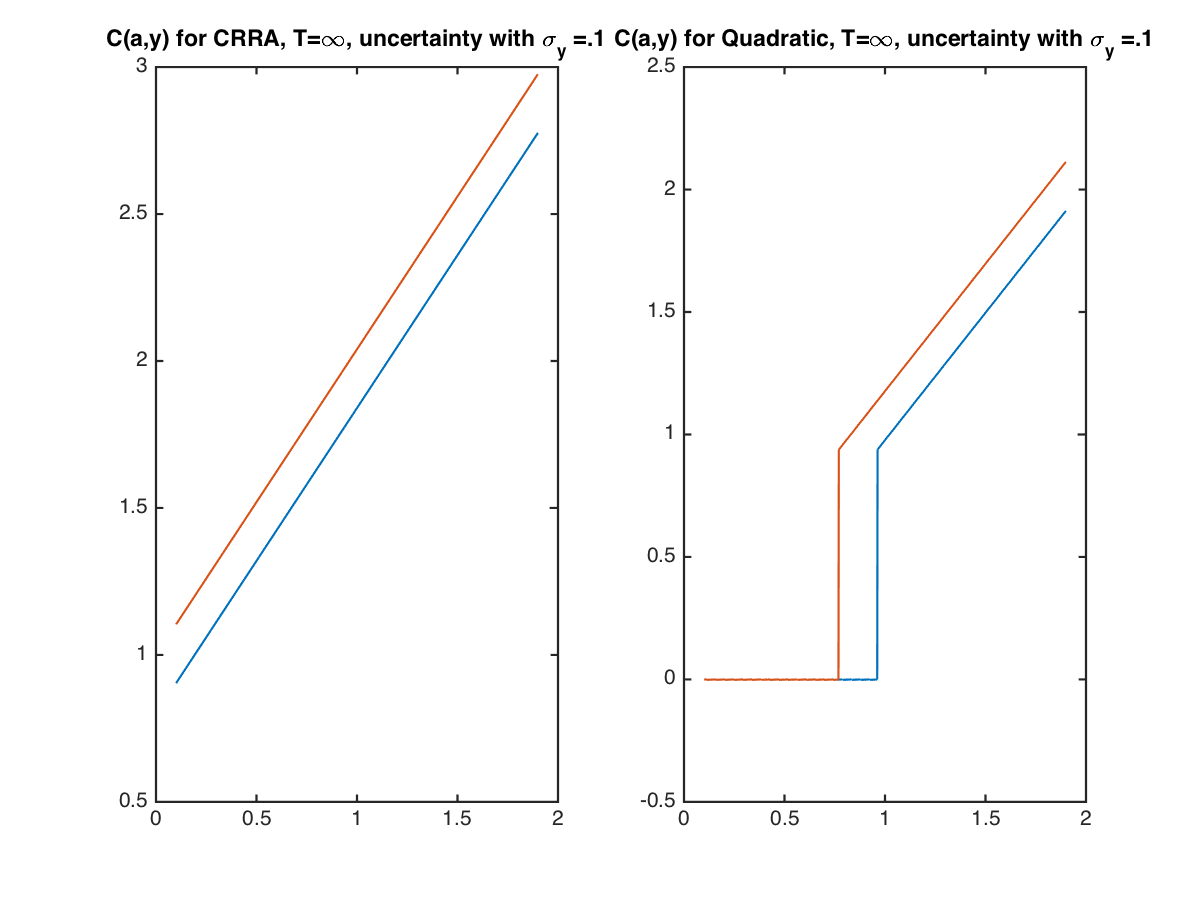
\includegraphics[width=\textwidth,height=8cm]{img/421a.png}
\caption{Q4-2a}\label{fig421a}
\end{figure}

This part just reduplicates the codes with letting $\sigma_y = 0.1$ hence it will generate two  policy functions w.r.t different shocks $y$for each different utility function shown in \ref{fig421a}

For infinite-lived household, with a small idiosyncratic risk, only happen thing is that when endowment is high (good shock), agents decide consume more and save in advance.
\begin{figure}[htbp]
\centering
\begin{minipage}[t]{0.48\textwidth}
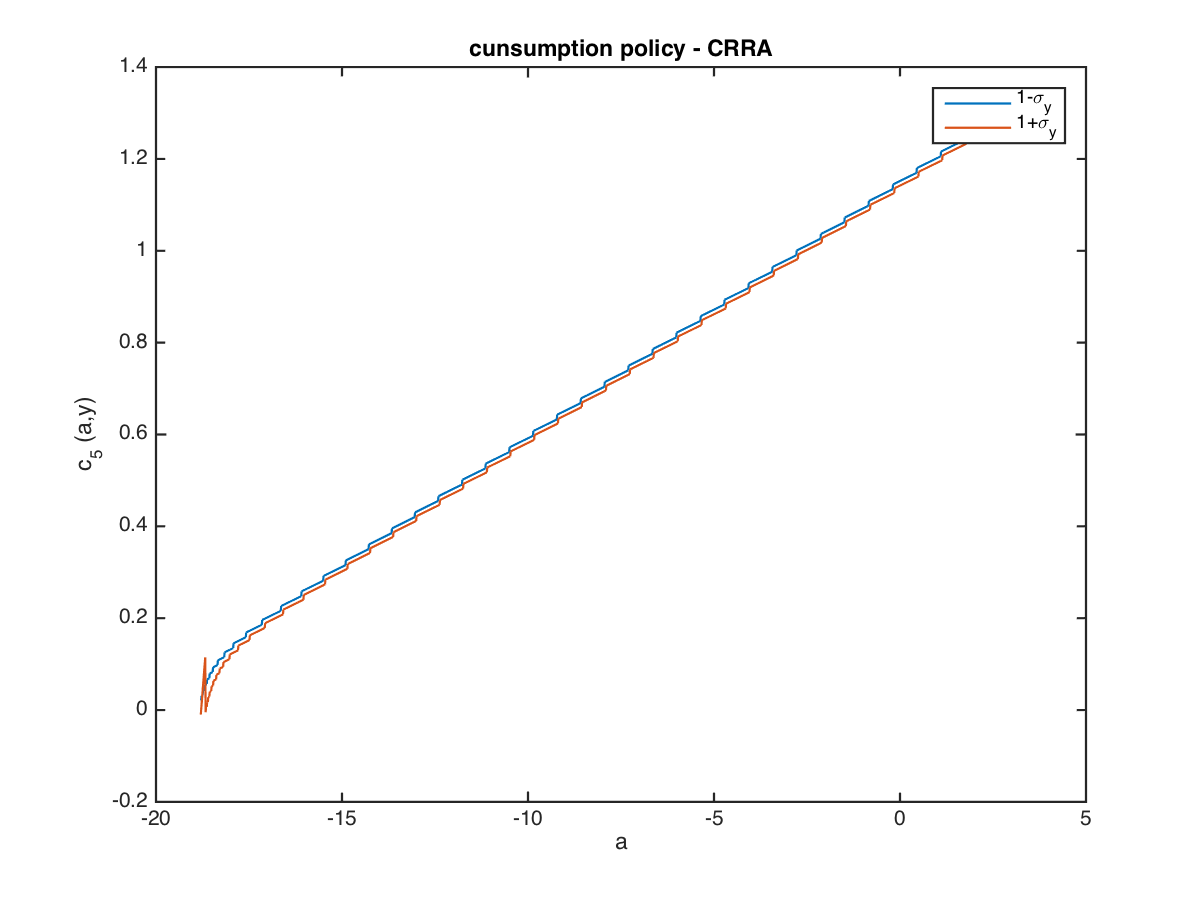
\includegraphics[width=\textwidth]{img/41fa.png}
\caption{Consumption policy function w.r.t different income risk - CRRA, finite}\label{fig41fa}
\end{minipage}
\begin{minipage}[t]{0.48\textwidth}
\centering
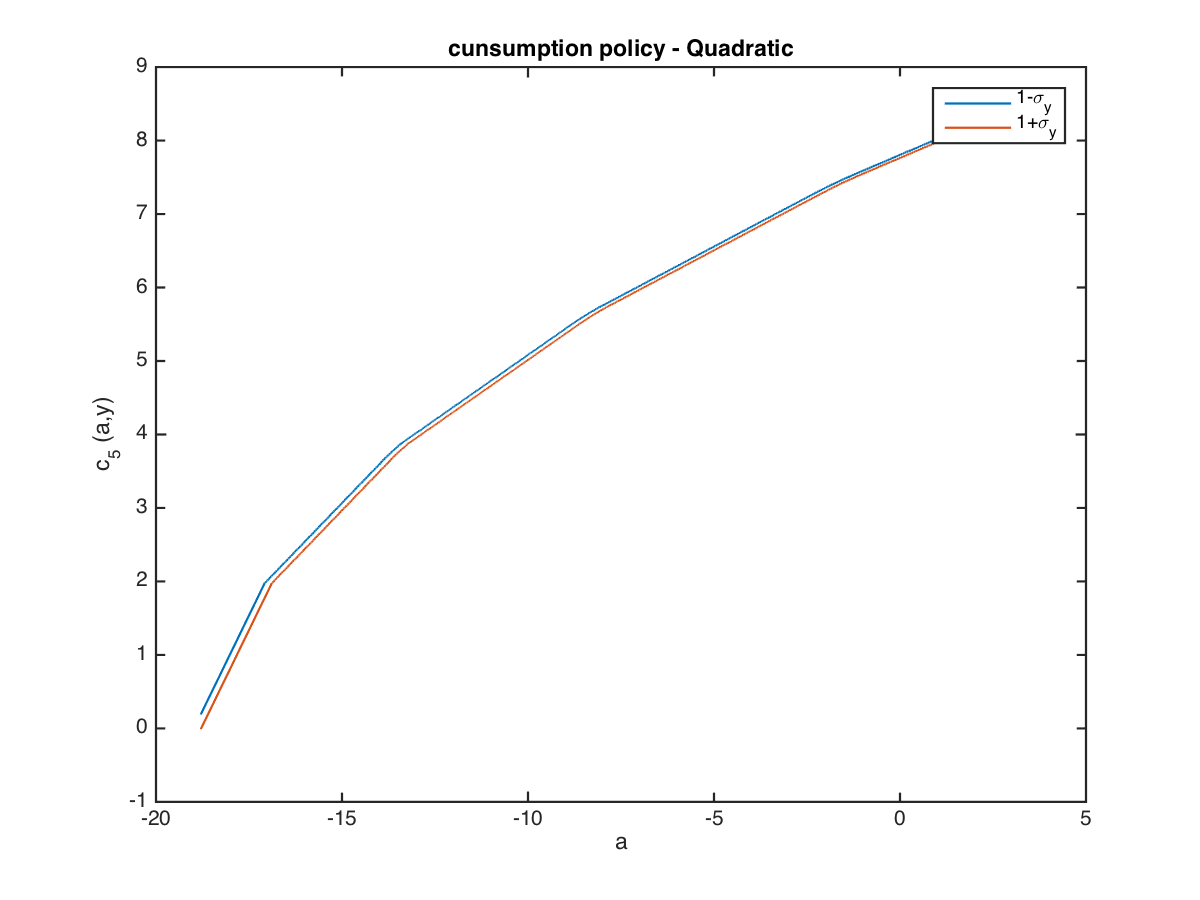
\includegraphics[width=\textwidth]{img/41qa.png}
\caption{Consumption policy function w.r.t different income risk - Quadratic, finite}\label{fig41qa}
\end{minipage}
\end{figure}

\medskip

\subsubsection{2. time path consumption plot for T = 45: Error: Oscillation}
Error is the  time path is extremely oscillation. Due to time limit, I will do this after due date.


\subsubsection{3. compare the case with $\sigma=2,5,20$}

once I made all the codes, for question 3 4 5, only  need to adjust the codes to specific parameters and compare, due to time limit, I will do this after due date. But just a very quick look at the consumption profile, we could with quadratic utility, agents consume much more in the beginning and get zeros later; but for CRRA utility, they could smooth consumption more better in order to consume in their old ages,and for larger $\sigma$, more prudence the agetns will become, hence, will consume more in their old ages (save more in younger ages), which is much more similar with the Asian style behavior. 

\begin{figure}[htbp]
\centering
\begin{minipage}[t]{0.48\textwidth}
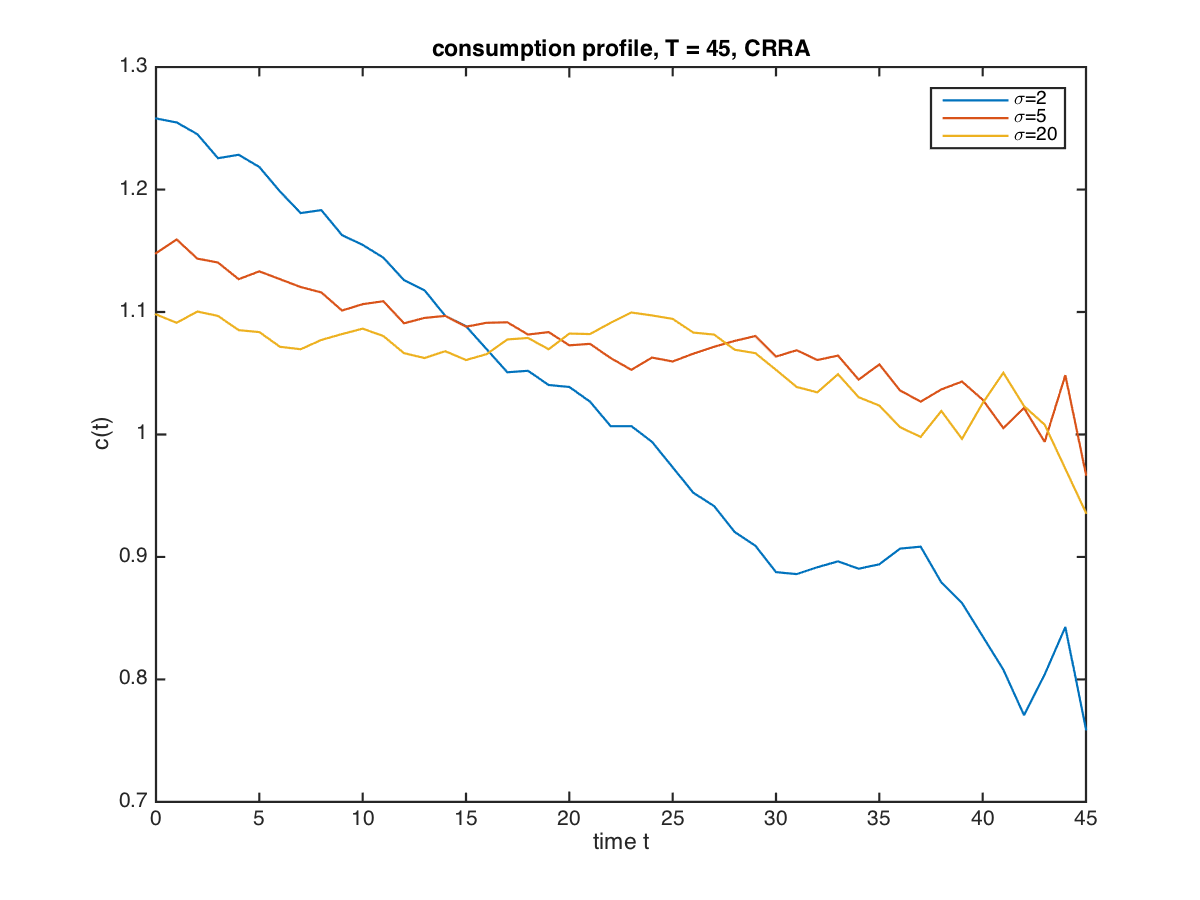
\includegraphics[width=\textwidth]{img/sigmacompare1.png}
\caption{Consumption time profile w.r.t different $\sigma$ - CRRA, finite}
\end{minipage}
\begin{minipage}[t]{0.48\textwidth}
\centering
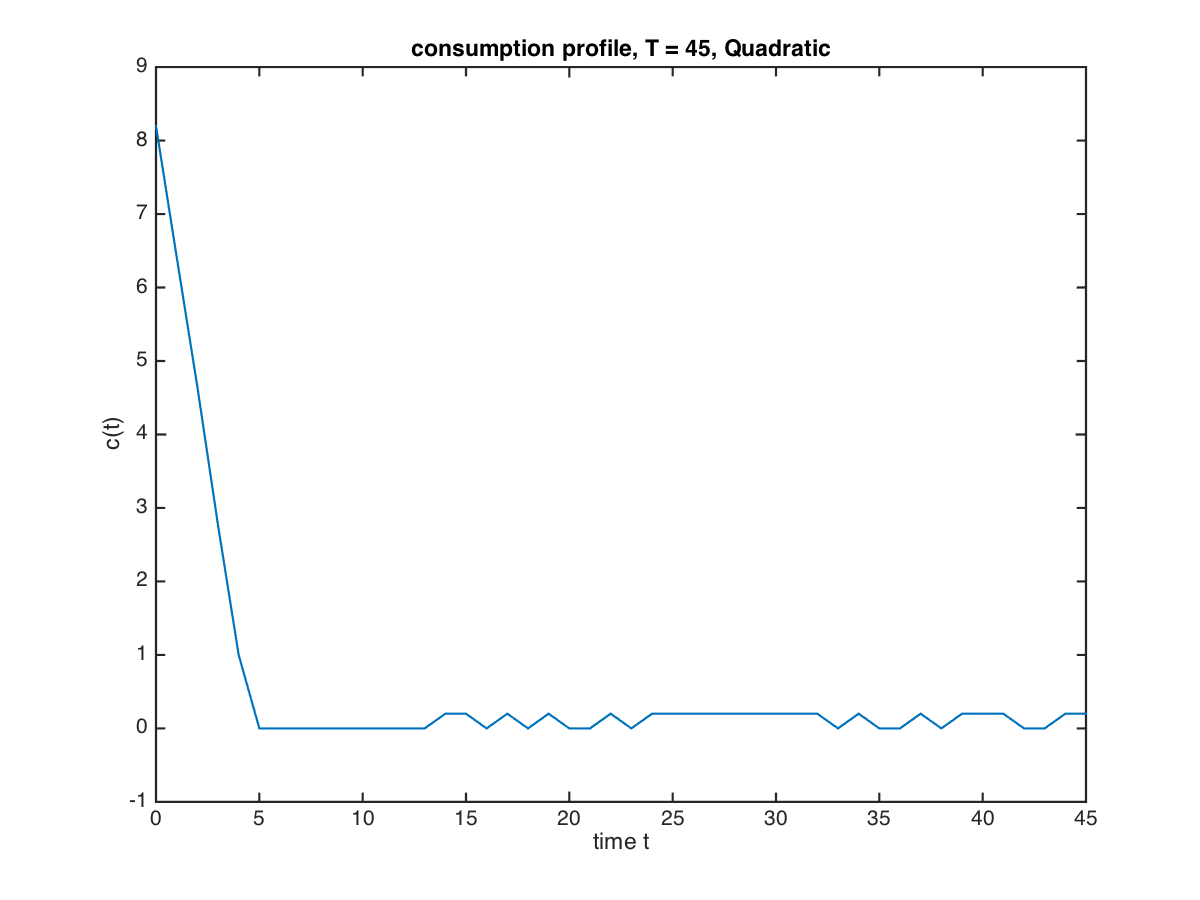
\includegraphics[width=\textwidth]{img/sigmacompare2.png}
\caption{Consumption time profile w.r.t different $\sigma$ - Quadratic, finite}
\end{minipage}
\end{figure}



\subsubsection{4. increase the variance of the income shock from .1 to .5}
Here, I set quadratic to certainty case, and CRRA to small uncertainty case, we could see that uncertainty could make decision different.

\begin{figure}[htbp]
\centering
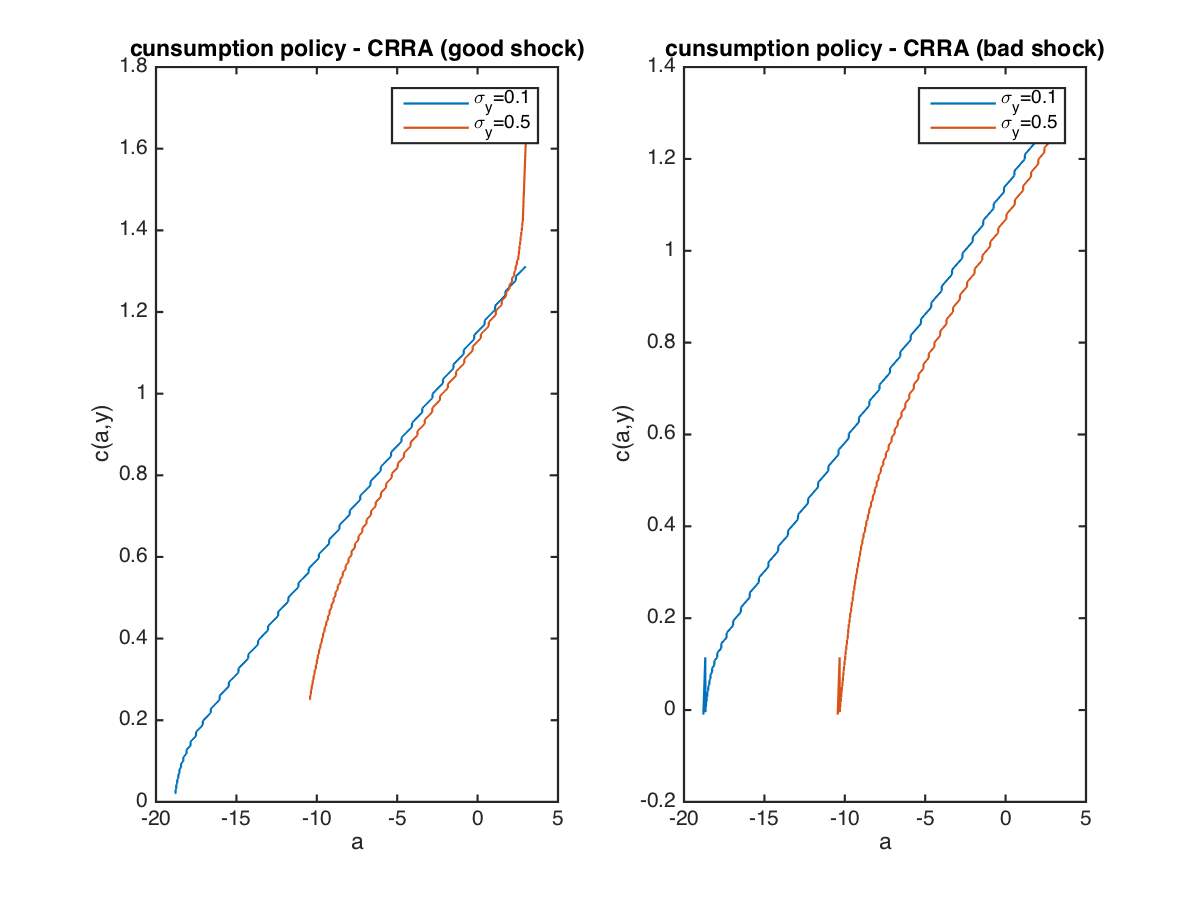
\includegraphics[width=\textwidth,height=8cm]{img/423.png}
\caption{increasing $\sigma_y = 0.1$ to $\sigma_y = 0.5$, CRRA, small uncertainty}
\end{figure}

\begin{figure}[htbp]
\centering
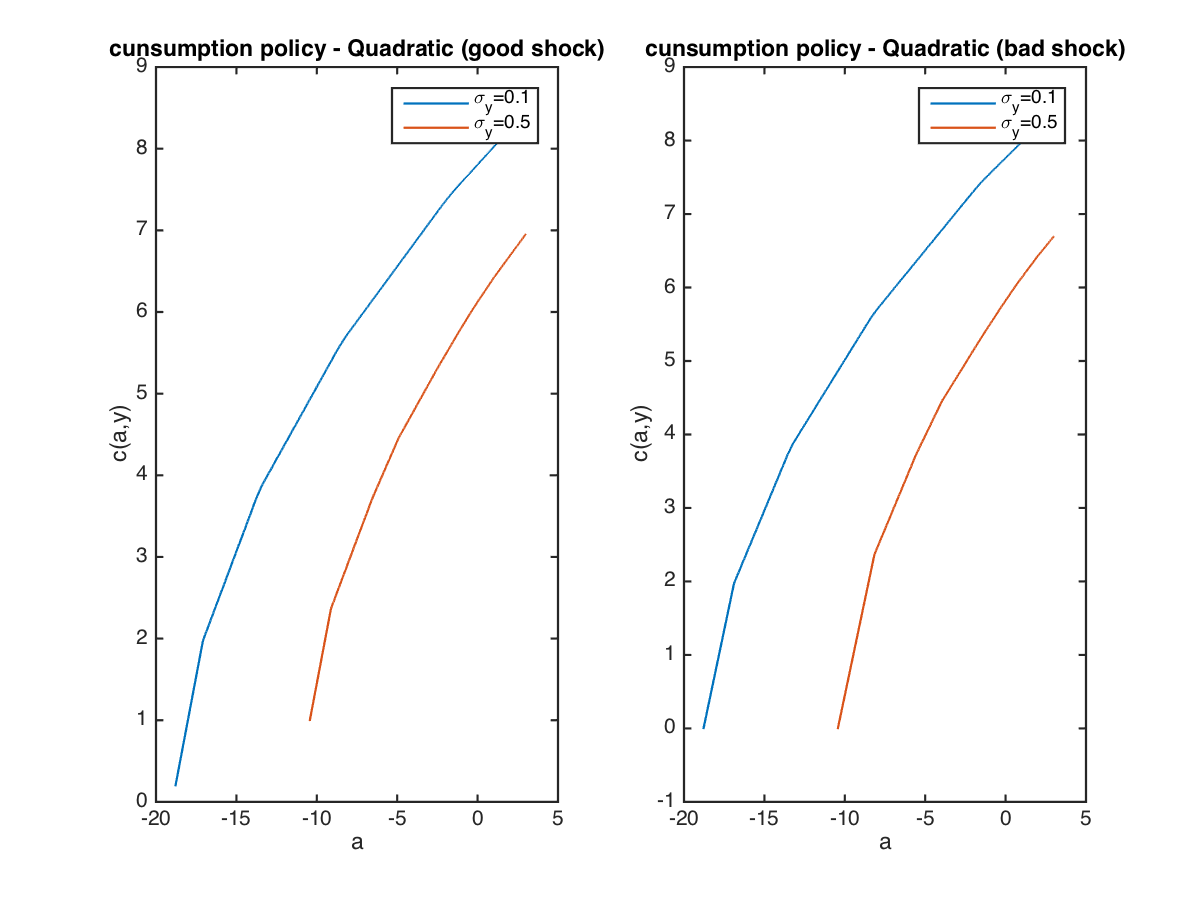
\includegraphics[width=\textwidth,height=8cm]{img/423-q.png}
\caption{increasing $\sigma_y = 0.1$ to $\sigma_y = 0.5$, Quadratic, no uncertainty}
\end{figure}

\subsubsection{5. increase the persistence of the income shock from 0 to .95}
By keeping $\sigma_y=0.5$, due to the time limit, here I only try the CRRA finite case, because the others are the same way to do.

\begin{figure}[htbp]
\centering
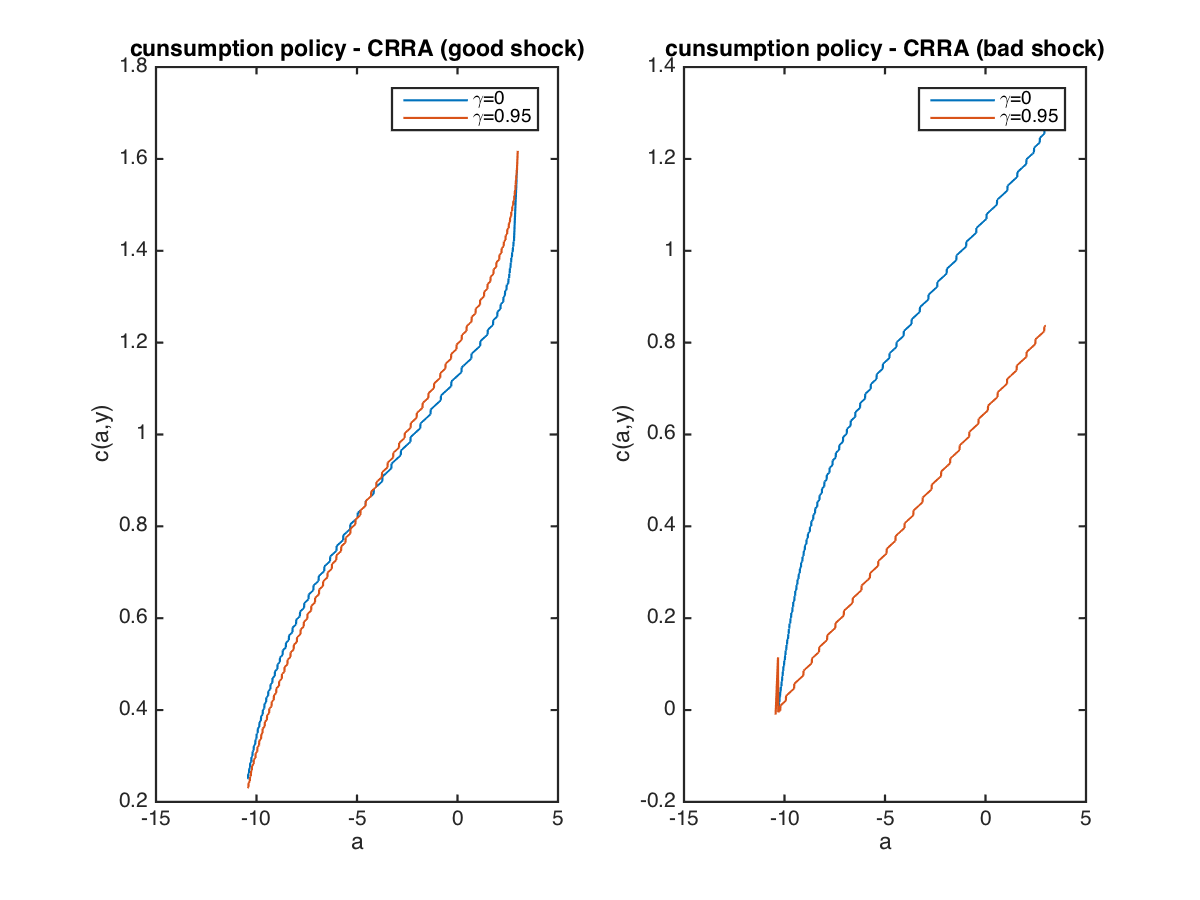
\includegraphics[width=\textwidth,height=8cm]{img/425.png}
\caption{increasing $\gamma = 0$ to $\gamma= 0.95$, CRRA, uncertainty $\sigma_y=0.5$}
\end{figure}





%%%%%%%%%%%%% Q.5 %%%%%%%%%%%
\pagebreak
\section{II.5 General Equilibrium}
\subsection{II.5.1 The simple ABHI model}

Following the Algorithm shown in our PS 5, and noted that there're already many source codes on the Internet, so this could be easily done with modifying existing codes and my previous codes.

Additional note:

By Luis's 2nd lecture, for computing General Equilibrium in this question, the key thing is, based on VFI, but to pin down the interest rate (r) and asset level (K) such that market is clearing  by checking demand side (firm) and supply side (households) to be equal:

\[ a' = g(a,y)\]
\[ K^{s} = \int_{a}^{\infty} \sum_{y\in Y}g(a,y)\Gamma (a,y) da \]
where: \[ \Gamma (\tilde{a},\tilde{y}) = \int_{\tilde{a}=g(a,y)} \sum_{y\in Y}\Gamma (a,y) \Pi (\tilde{y}|y)da \text{, for every } \tilde{a}, \tilde{y} \in A \times Y \]  


By a rough look at the Chapter 11, Handbook of Macroeconomics, written by Krueger Mitman and Perri, I found out that they use different parameter values compared to our PS5, hence, fit the data is not possible for our case. i.e. KMP paper uses $\beta=0.9899, \sigma=1$ but we use $\beta=0.9434, \sigma=2$.
First, when computing our type of model, I obtain the corresponding distribution of consumption, wealth and income as follows: \footnote{when increasing asset grid size, becomes more oscillation and polarized}

\begin{figure}[htbp]
\centering
\begin{minipage}[t]{0.48\textwidth}
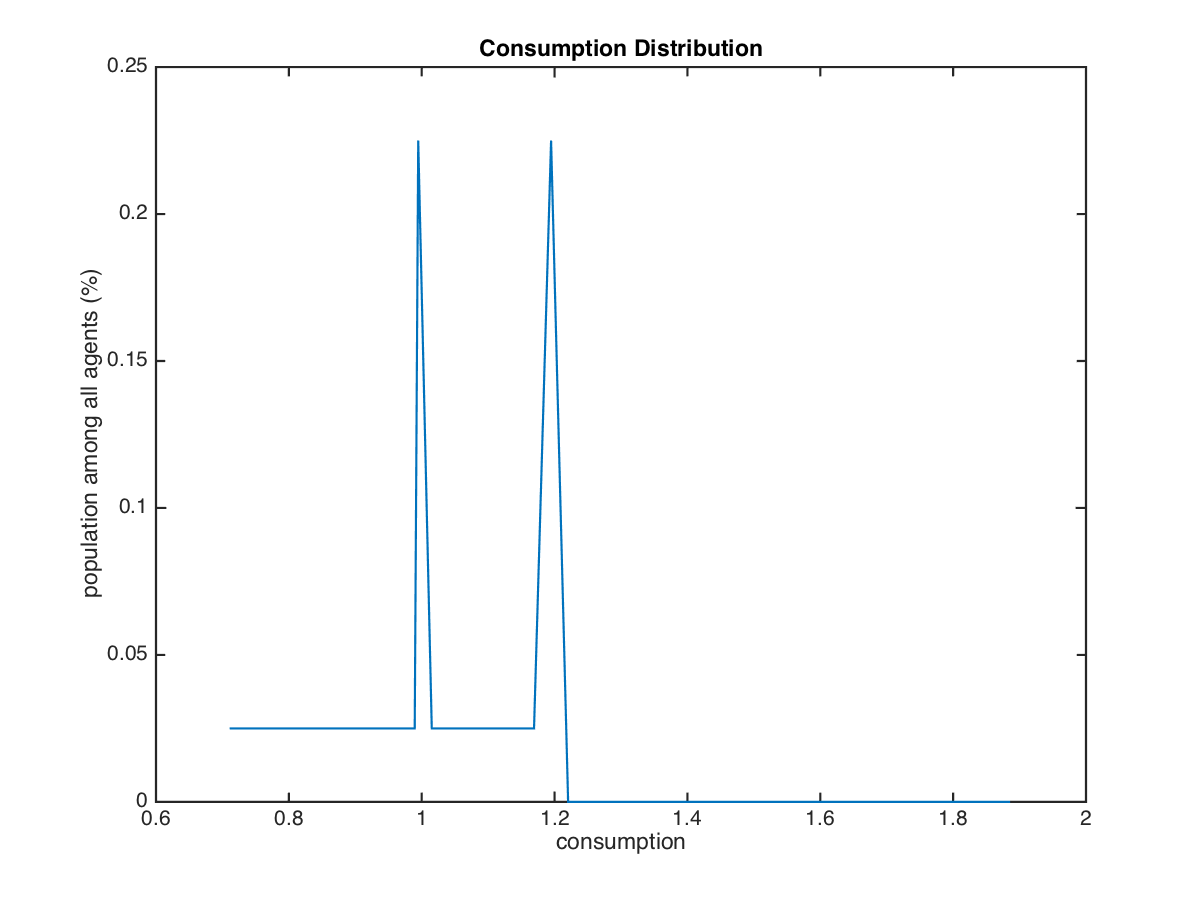
\includegraphics[width=\textwidth]{img/consumdist.png}
\end{minipage}

\begin{minipage}[t]{0.48\textwidth}
\centering
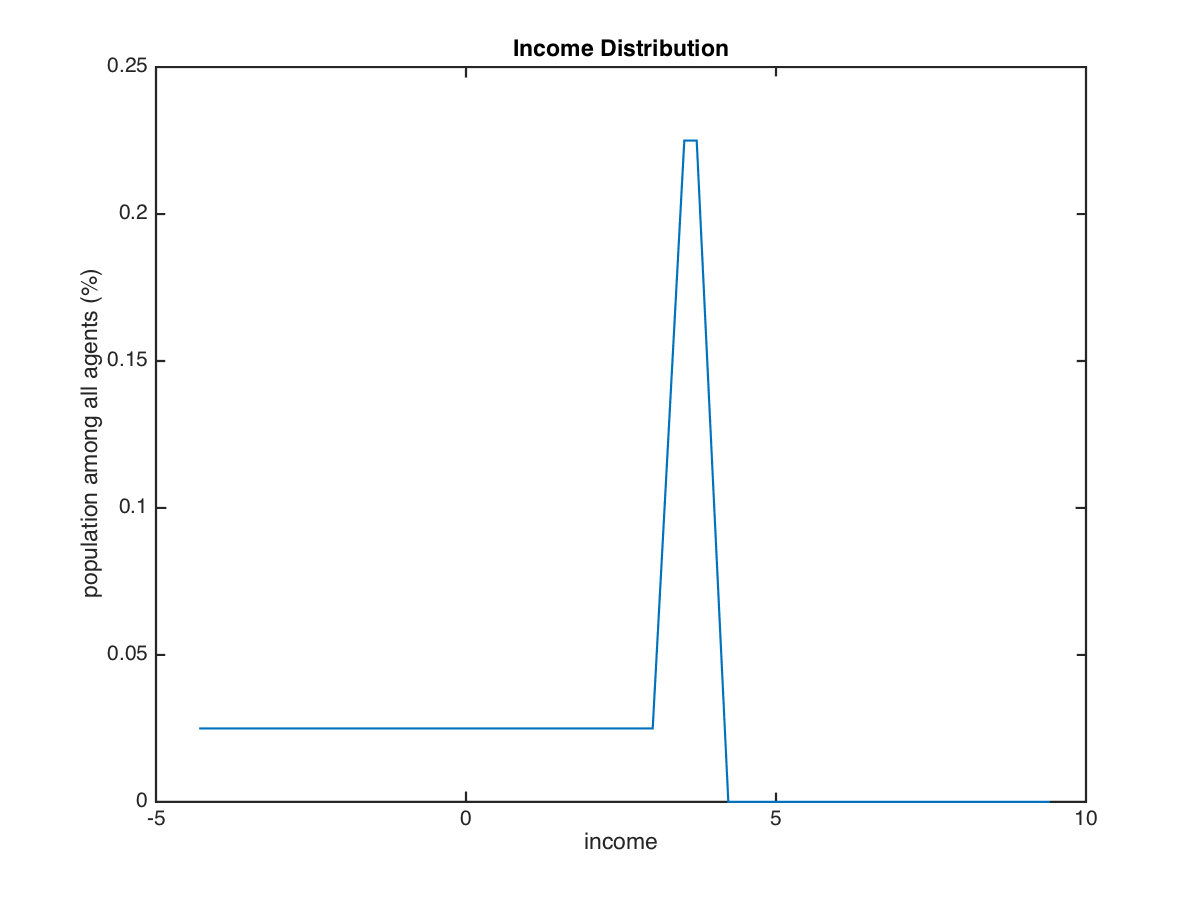
\includegraphics[width=\textwidth]{img/incomedist.png}
\end{minipage}

\begin{minipage}[t]{0.48\textwidth}
\centering
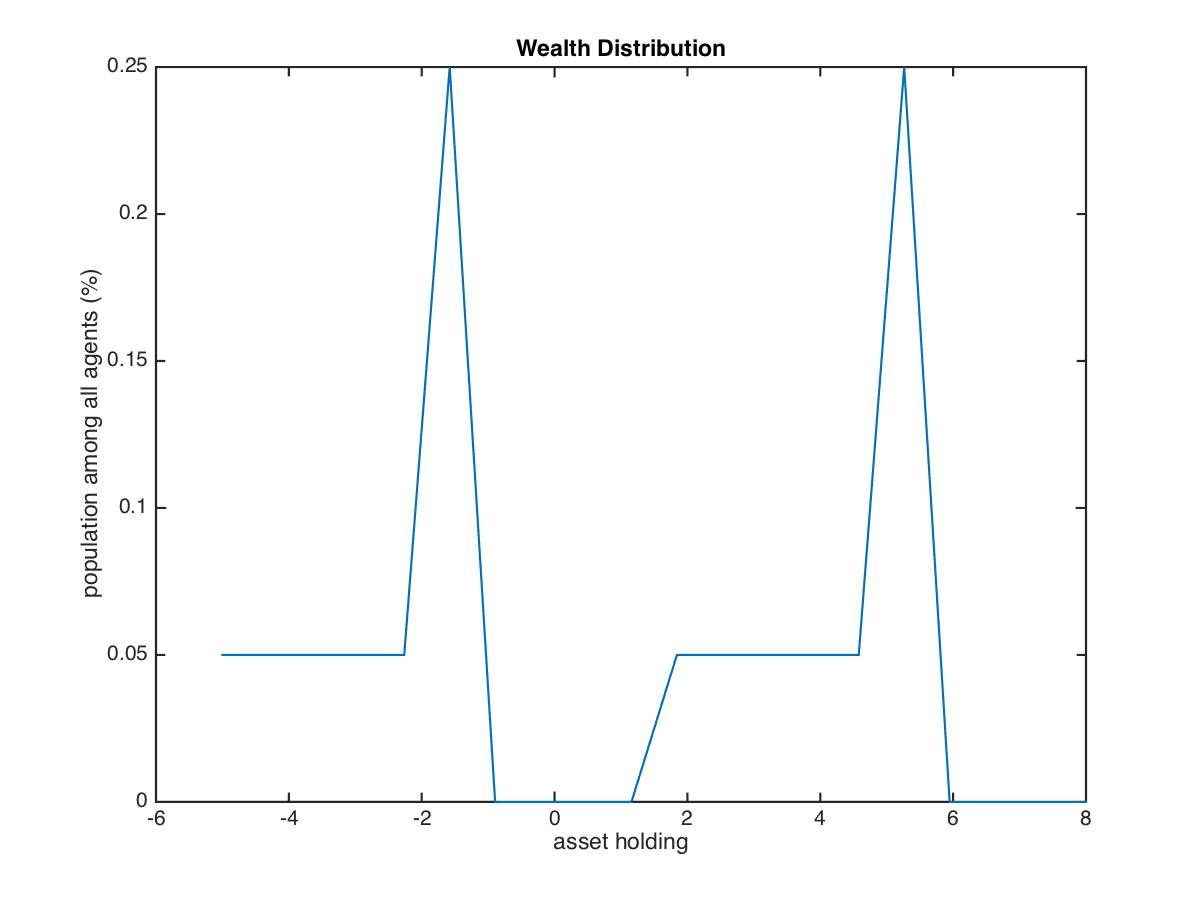
\includegraphics[width=\textwidth]{img/wealthdist.png}
\end{minipage}
\caption{Consumption, Income, Wealth Distribution, CRRA $\sigma=2$,$\sigma_y=0.1$, asset grid size: 20}
\end{figure}

\begin{figure}[htbp]
\centering
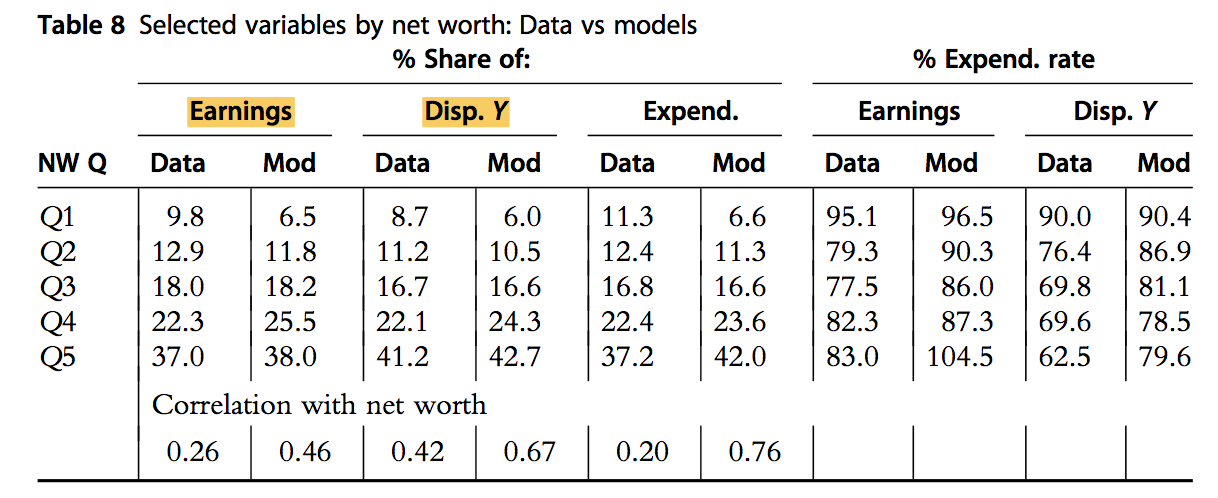
\includegraphics[width=0.68\textwidth]{img/table8.png}
\caption{Handbook of Macroeconomics, Chapter 11, table 8}\label{fig41qa}
\end{figure}

Second, I compute the quantile for my simulation and compared to KMP paper (which I think is meaningless)

% Please add the following required packages to your document preamble:
% \usepackage{booktabs}
\begin{table}[htbp]
\centering
\begin{tabular}{@{}ccccc@{}}
\toprule
     & \multicolumn{4}{c}{\% Share of:}                                   \\ \midrule
     & \multicolumn{2}{c}{Earnings (Wealth)} & \multicolumn{2}{c}{Income} \\
NW Q & KMP             & my model            & KMP        & my model      \\
Q1   & 6.5             & 20.75               & 8.7        & 12.5          \\
Q2   & 11.8            & 29.25               & 10.5       & 27.5          \\
Q3   & 18.2            & 12.26               & 16.6       & 7.5           \\
Q4   & 25.5            & 37.74               & 24.3       & 27.5          \\
Q5   & 38.0            & 0                   & 42.7       & 0             \\ \bottomrule
\end{tabular}
\end{table}


\pagebreak
\subsection{II.5.2 Solving Aiyagari (1994)}
By the same operations like previous section, we could obtain the relevant distribution for Aiyagari model, by straightly using my previous codes(no firm no capital model), changing the parameter values to Aiyagari(1994) set-up, we can obtain the following (maintain the grid number equals to 20):

\begin{figure}[htbp]
\centering
\begin{minipage}[t]{0.48\textwidth}
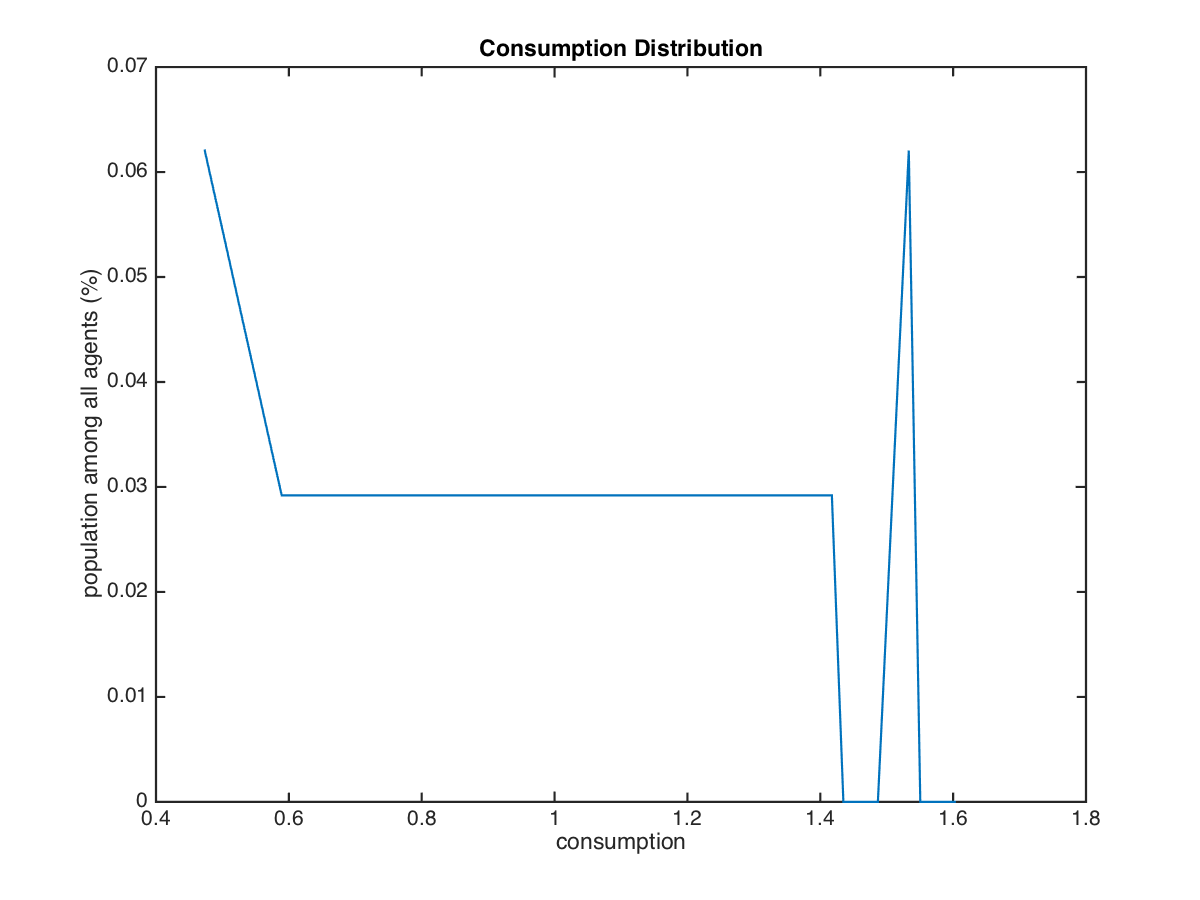
\includegraphics[width=\textwidth]{img/1consumdist.png}
\end{minipage}

\begin{minipage}[t]{0.48\textwidth}
\centering
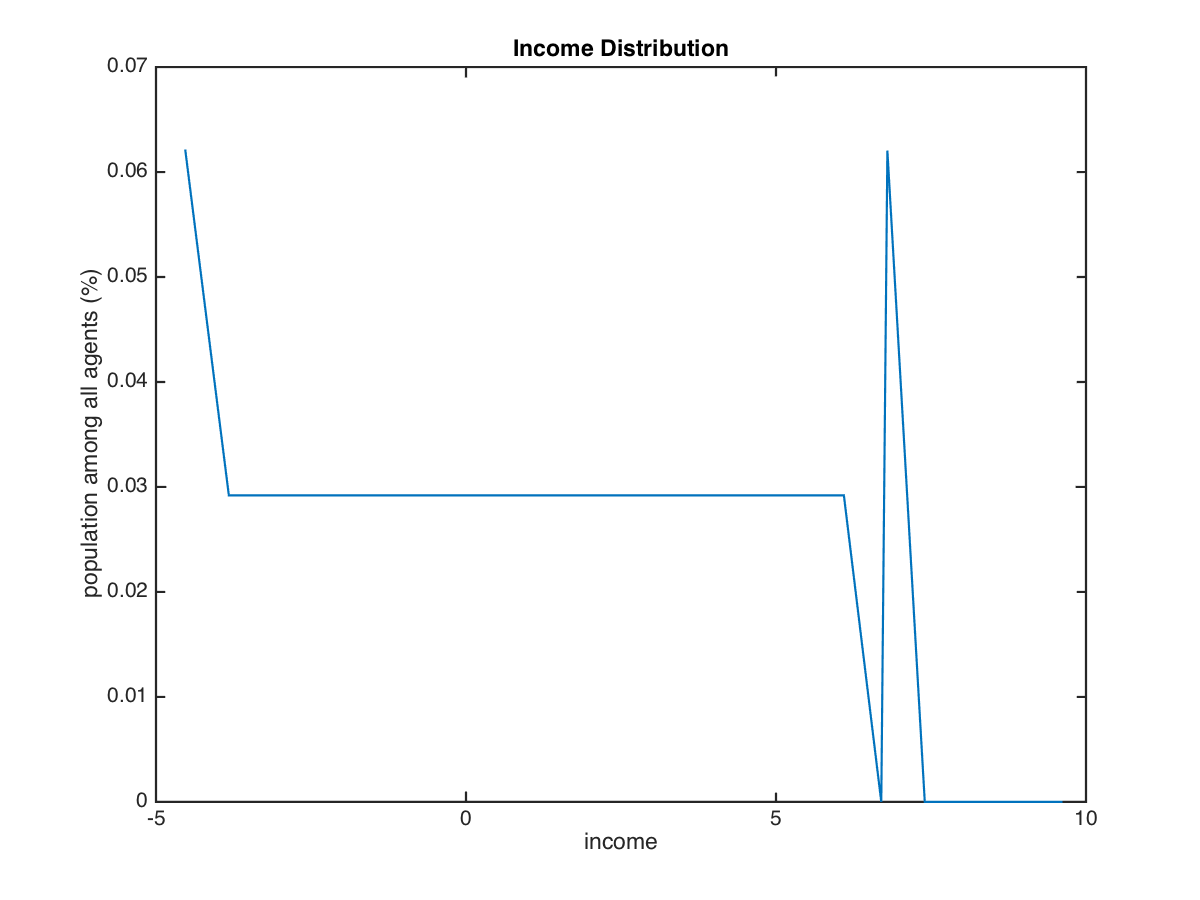
\includegraphics[width=\textwidth]{img/1incomedist.png}
\end{minipage}

\begin{minipage}[t]{0.48\textwidth}
\centering
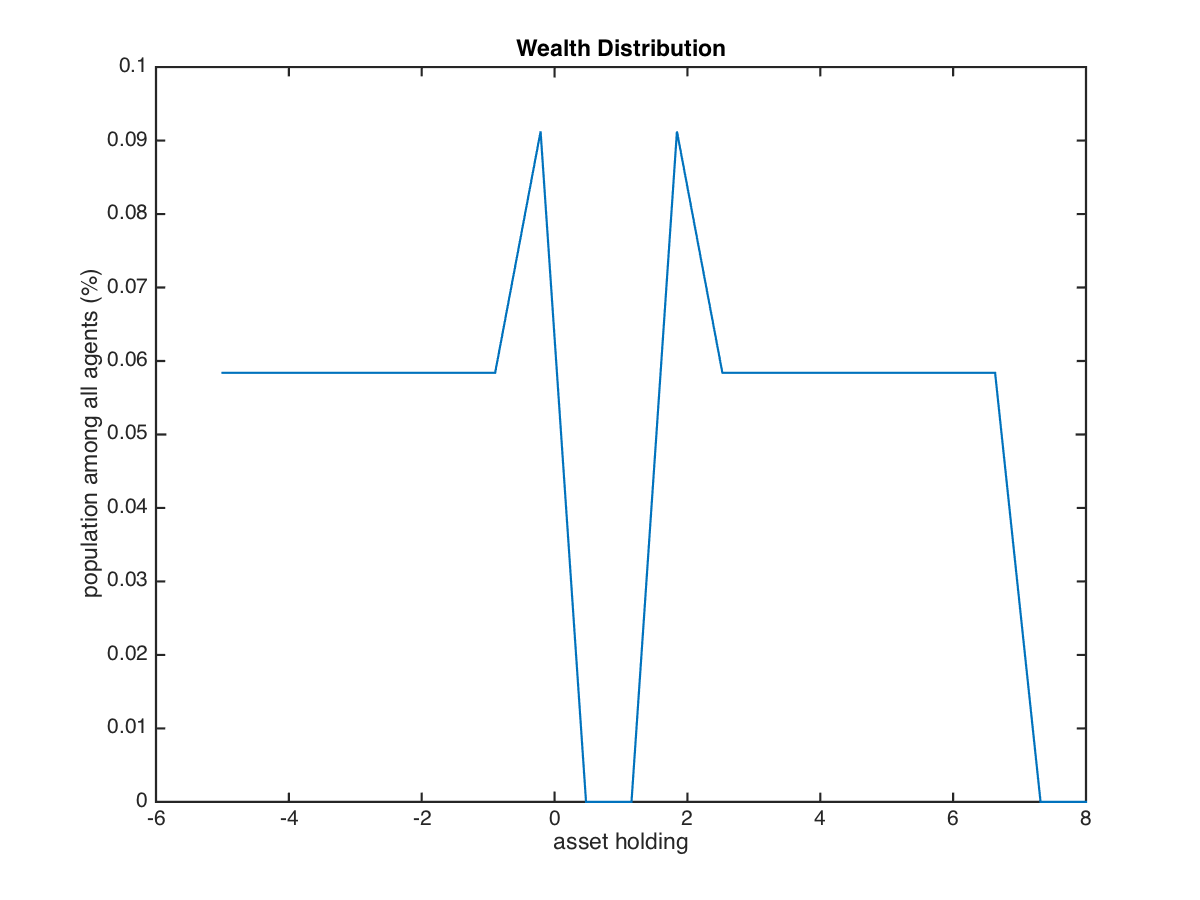
\includegraphics[width=\textwidth]{img/1wealthdist.png}
\end{minipage}
\caption{Consumption, Income, Wealth Distribution, Aiyagari(1994) parameters, asset grid size: 20}
\end{figure}

However, if we wanna fit the KMP results or PSID data more closer, by using joint Markov, or adding firm sector in our model, we could obtain a downright-decreasing distribution such as the following:

\begin{figure}[htbp]
\centering
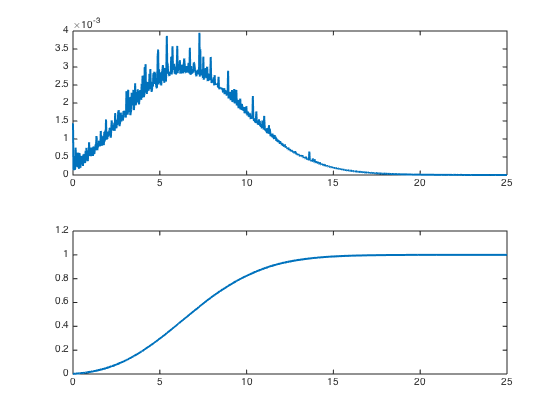
\includegraphics[width=0.68\textwidth]{img/1111.png}
\caption{Capital Distribution from a more reasonable set-up Aiyagari(1994) model}
\end{figure}

\pagebreak
\subsection{II.5.3 An application}
\textit{Modify your economy in (II.5.2) to an overlapping generations economy. Add a unitary household model with men and women that share household consumption. Men work inelastically and women face a labor choice (intensive margin). At each period, the household decide whether to put effort in getting a child or not, which is the outcome of a probabilistic function that depends on this effort. This function replicates the rapid decline in women fecundity after age 35. Children are costly in goods and time until they leave the household, but they provide utility when they are around.}

\subsubsection{Describe your economic environment (preferences, technology and market structure)}

reference: \textit{Jeremy Greenwood \& Nezih Guner \& Guillaume Vandenbroucke, 2015. "Family Economics Writ Large," Economie d'Avant Garde Research Reports 26, Economie d'Avant Garde.}

Now, under the framework of Overlapping Generation, we aim to solve the life-cycle problem of a family (a man and a woman), hence maximizing a weighted sum of utility of two persons, and consumption altogether shown in the budget constraint.

The household’s utility function is: 

\begin{align}
V^{early}(w_f,w_m,\lambda)&=\alpha ln(w_m l_m + w_f l_f) + (1-\alpha)ln(1-l_m-l_c) + (1-\alpha)ln(1-l_f-l_c) + \lambda -\phi ln(e)\\
&+ \beta [\alpha ln(w_m l^2_m + w_f l^2_f) + (1-\alpha)ln(1-l^2_m) + (1-\alpha)ln(1-l^2_f) ] \\
\medskip
V^{late}(w_f,w_m,\lambda) &= \alpha ln(w_m l_m + w_f l_f) + (1-\alpha)ln(1-l_m) + (1-\alpha)ln(1-l_f)\\
&+ \beta [\alpha ln(w_m l^2_m + w_f l^2_f) + (1-\alpha)ln(1-l^2_m-l_c) + (1-\alpha)ln(1-l^2_f-l_c) + \pi (\lambda -\phi ln(e))] 
\end{align}

where, 

$\pi$ measures the fecundity, hence show up at second period if they want to have children;

$\lambda$ brings the positive utility for household;

$-\phi ln(e)$ measures the efforts household put on the children bearing;

$l_c$ measures the time cost of children. 

\subsubsection{stay tuned}


\end{document}